\documentclass[11pt]{beamer}
\usepackage{listings} % Include the listings-package
\usepackage[T1]{fontenc}
\usepackage[utf8]{inputenc}
\usepackage[english]{babel}
\usepackage{amsmath}
\usepackage{amssymb, amsfonts, latexsym, cancel}
\usepackage{float}
\usepackage{graphicx}
\usepackage{epstopdf}
\usepackage{subfigure}
\usepackage{hyperref}
%\usepackage{authblk}
\usepackage{blindtext}
\usepackage{booktabs} % Allows the use of \toprule, 
\usepackage{filecontents}
\usepackage{courier} %% Sets font for listing as Courier.
\usepackage{listings}
%\usepackage{listings, xcolor}
\lstset{
tabsize = 2, %% set tab space width
showstringspaces = false, %% prevent space marking in strings, string is defined as the text that is generally printed directly to the console
numbers = left, %% display line numbers on the left
commentstyle = \color{green}, %% set comment color
keywordstyle = \color{blue}, %% set keyword color
stringstyle = \color{red}, %% set string color
rulecolor = \color{black}, %% set frame color to avoid being affected by text color
basicstyle = \small \ttfamily , %% set listing font and size
breaklines = true, %% enable line breaking
numberstyle = \tiny,
}
\usepackage{caption}
\DeclareCaptionFont{white}{\color{white}}
\DeclareCaptionFormat{listing}{\colorbox{gray}{\parbox{\textwidth}{#1#2#3}}}
\captionsetup[lstlisting]{format=listing,labelfont=white,textfont=white}
\definecolor{urlColor}{rgb}{0.06, 0.3, 0.57}
\definecolor{linkColor}{rgb}{0.57, 0.0, 0.04}
\definecolor{fileColor}{rgb}{0.0, 0.26, 0.26}
\hypersetup{
    colorlinks=true,
    linkcolor=linkColor,
    filecolor=fileColor,      
    urlcolor=urlColor,
}
\urlstyle{same}
\setbeamercovered{transparent}
%\usetheme{Boadilla}
\usetheme{CambridgeUS}
%\usetheme{Berkeley}
%\usetheme{Warsaw}
%\usetheme{Madrid}

\title[Prototipado en Papel]{\bf\Huge Prototipado en Papel}


\author[rescobedoq]
{
    Alvan Ventura Edsel Yael \inst{1}\\
	Chuctaya Ruiz Diego Moises \inst{2}\\
	Esteba Cruz Santos Adilson\inst{3}\\
	Ramos Ticona Gilbert Will\inst{4}
}
\institute[UNSA]
{
\inst{1}% 
System Engineering School\\
}
\date[2020-10-10]{\scriptsize{2020-10-10}}
%\logo{
\includegraphics[width=3.0cm]{img/logo_unsa.jpg}}
\titlegraphic{
\includegraphics[width=3.0cm]{logo_unsa.jpg}}
\begin{document}

\begin{frame}
\titlepage
\end{frame}

\begin{frame}
\frametitle{Content}
\tableofcontents
\end{frame}

\section{Brainstorm}
\begin{frame}
\frametitle{Brainstorm}
\begin{itemize}
 \item La lluvia de ideas nos ayudó a ver las mejores ideas de cada integrante.
 \item Nos preguntamos cuál es el contexto y sus necesidades disponible del usuario.

\begin{figure}[t]

\includegraphics[width=4cm, height=4cm]{lluvia.png}
\centering
\end{figure}
\end{itemize}
\end{frame}

\section{Identificar caracteristicas y contenido}
%References frame
\begin{frame}
\frametitle{Identificar caracteristicas y contenido}
\begin{itemize}
\item  Aqui enumeramos todas las funciones y el contenido que queremos que esten disponibles para el usuario. 
%santos usa el enumerate
\item  Debe tener una opción para registrarse.
\item  Habilitar la personalización del perfil del usuario.
\item  Fomentar el uso del contenido en línea por parte de los clientes.
\item  Consideraciones sobre la experiencia del usuario (centrado en los usuarios).
\item  El proceso de descarga.
\item  El cambio entre múltiples temas.
\item  La navegación del tema y sus contenidos.
\item  Debe tener un historial de las victorias y derrotas de Alianza Lima.

\end{itemize}
\end{frame}

%References frame
\section{Objetivos del Cliente}
\begin{frame}
\frametitle{Objetivos del cliente}
\begin{itemize}
\item El cliente espera poder ver lo próximos partidos de su equipo favorito
\item El cliente espera poder ver los mejores goles de su equipo.
\item Comprobación de los titulares de noticias del equipo
\item Comprobación de una noticia individual
\item Comprobando los próximos partidos del equipo
\item Comprobación de la posición y los resultados del equipo en la tabla de la liga
\item El cliente podrá ver las probabilidades estadísticas de cada equipo 

\end{itemize}
\end{frame}

%References frame
\section{Secciones de contenido}
\begin{frame}
\frametitle{Secciones de contenido}

%\textbf{Los cuatro principios del buen diseño de Donald Norman:}
    \item Enumeramos y decidimos las cuatro secciones prinicipales que deberia tener nuestro primer prototipo en papel:
%esto de qui
\begin{enumerate}
    \item Imagenes actuales del Equipo Alianza Lima.
    \item Informacion General del Equipo Alianza Lima.
    \item Historias del Equipo Alianza Lima.
    \item Actualizaciones de informacion del Equipo Alinza Lima.
\end{enumerate}
\end{frame}


\section{Primer Prototipo}
\begin{frame}{Primer Prototipo}
%\textcolor{red}{Compensaciones}\textbf{(El diseño es una serie de compensaciones)}
\begin{itemize}
    \item Comenzamos a ver el flujo de pantallas.
    \item Consideramos las secciones de contenido.
    \item Consideramos los objetivos del usuario, al entrar en nuestra aplicacion móvil. 
\end{itemize}
\begin{figure}[t]
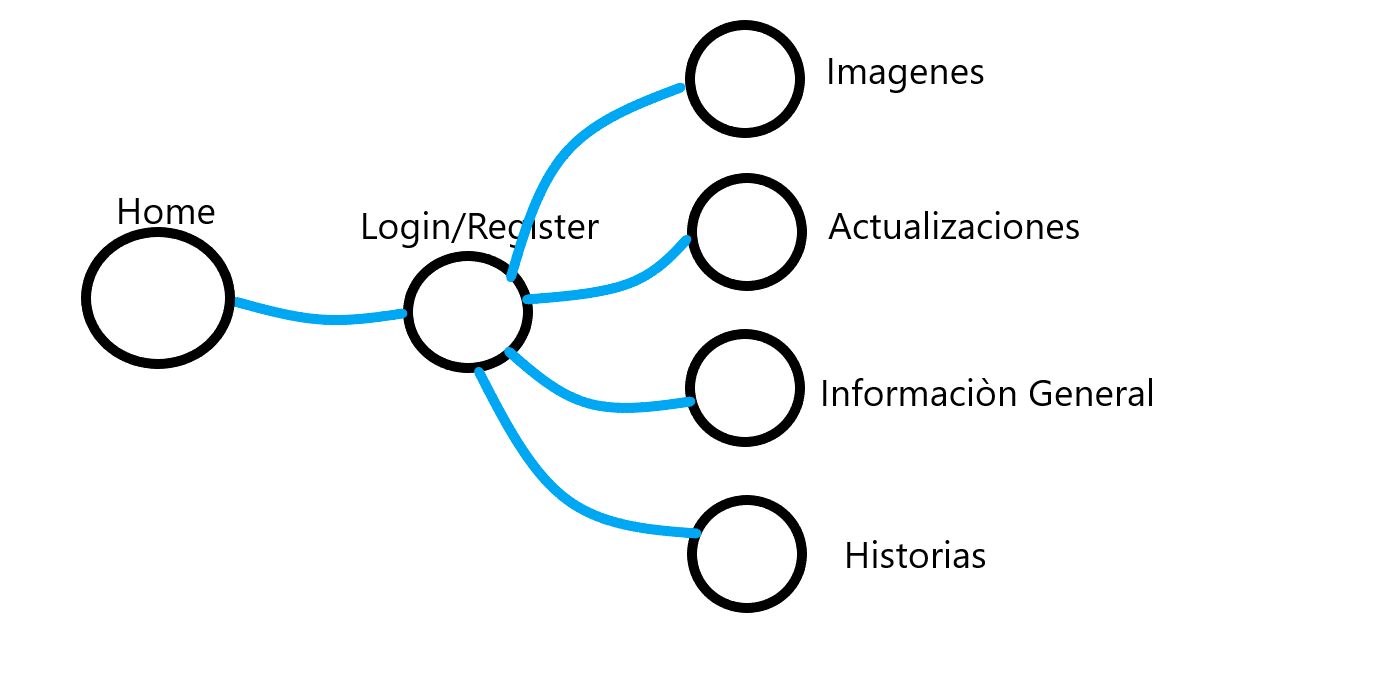
\includegraphics[width=9cm, height=5cm]{flujo.png}
\centering
\end{figure}
\end{frame}
\section{Imagenes del Equipo}
\begin{frame}{Imagenes del Equipo}

%\textcolor{red}{Prototipo TradeOff:}\textbf{ (Información vs tiempo)}
\begin{figure}
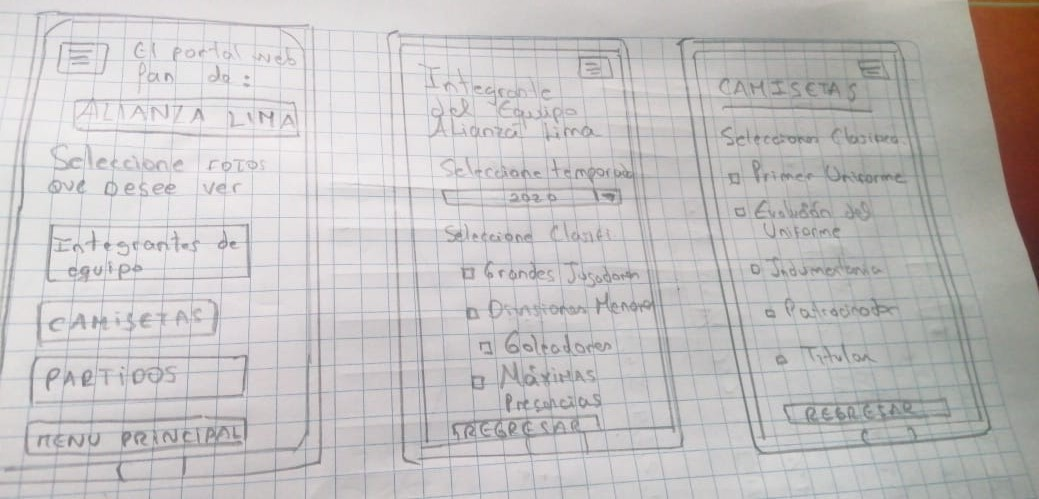
\includegraphics[width=\linewidth]{interfaces1.jpeg}
\centering
\end{figure}
\end{frame}
\section{Informacion General}
\begin{frame}{Informacion General}
%\textcolor{red}{Prototipo TradeOff:}\textbf{ (Información vs tiempo)}
\begin{figure}
 \centering
   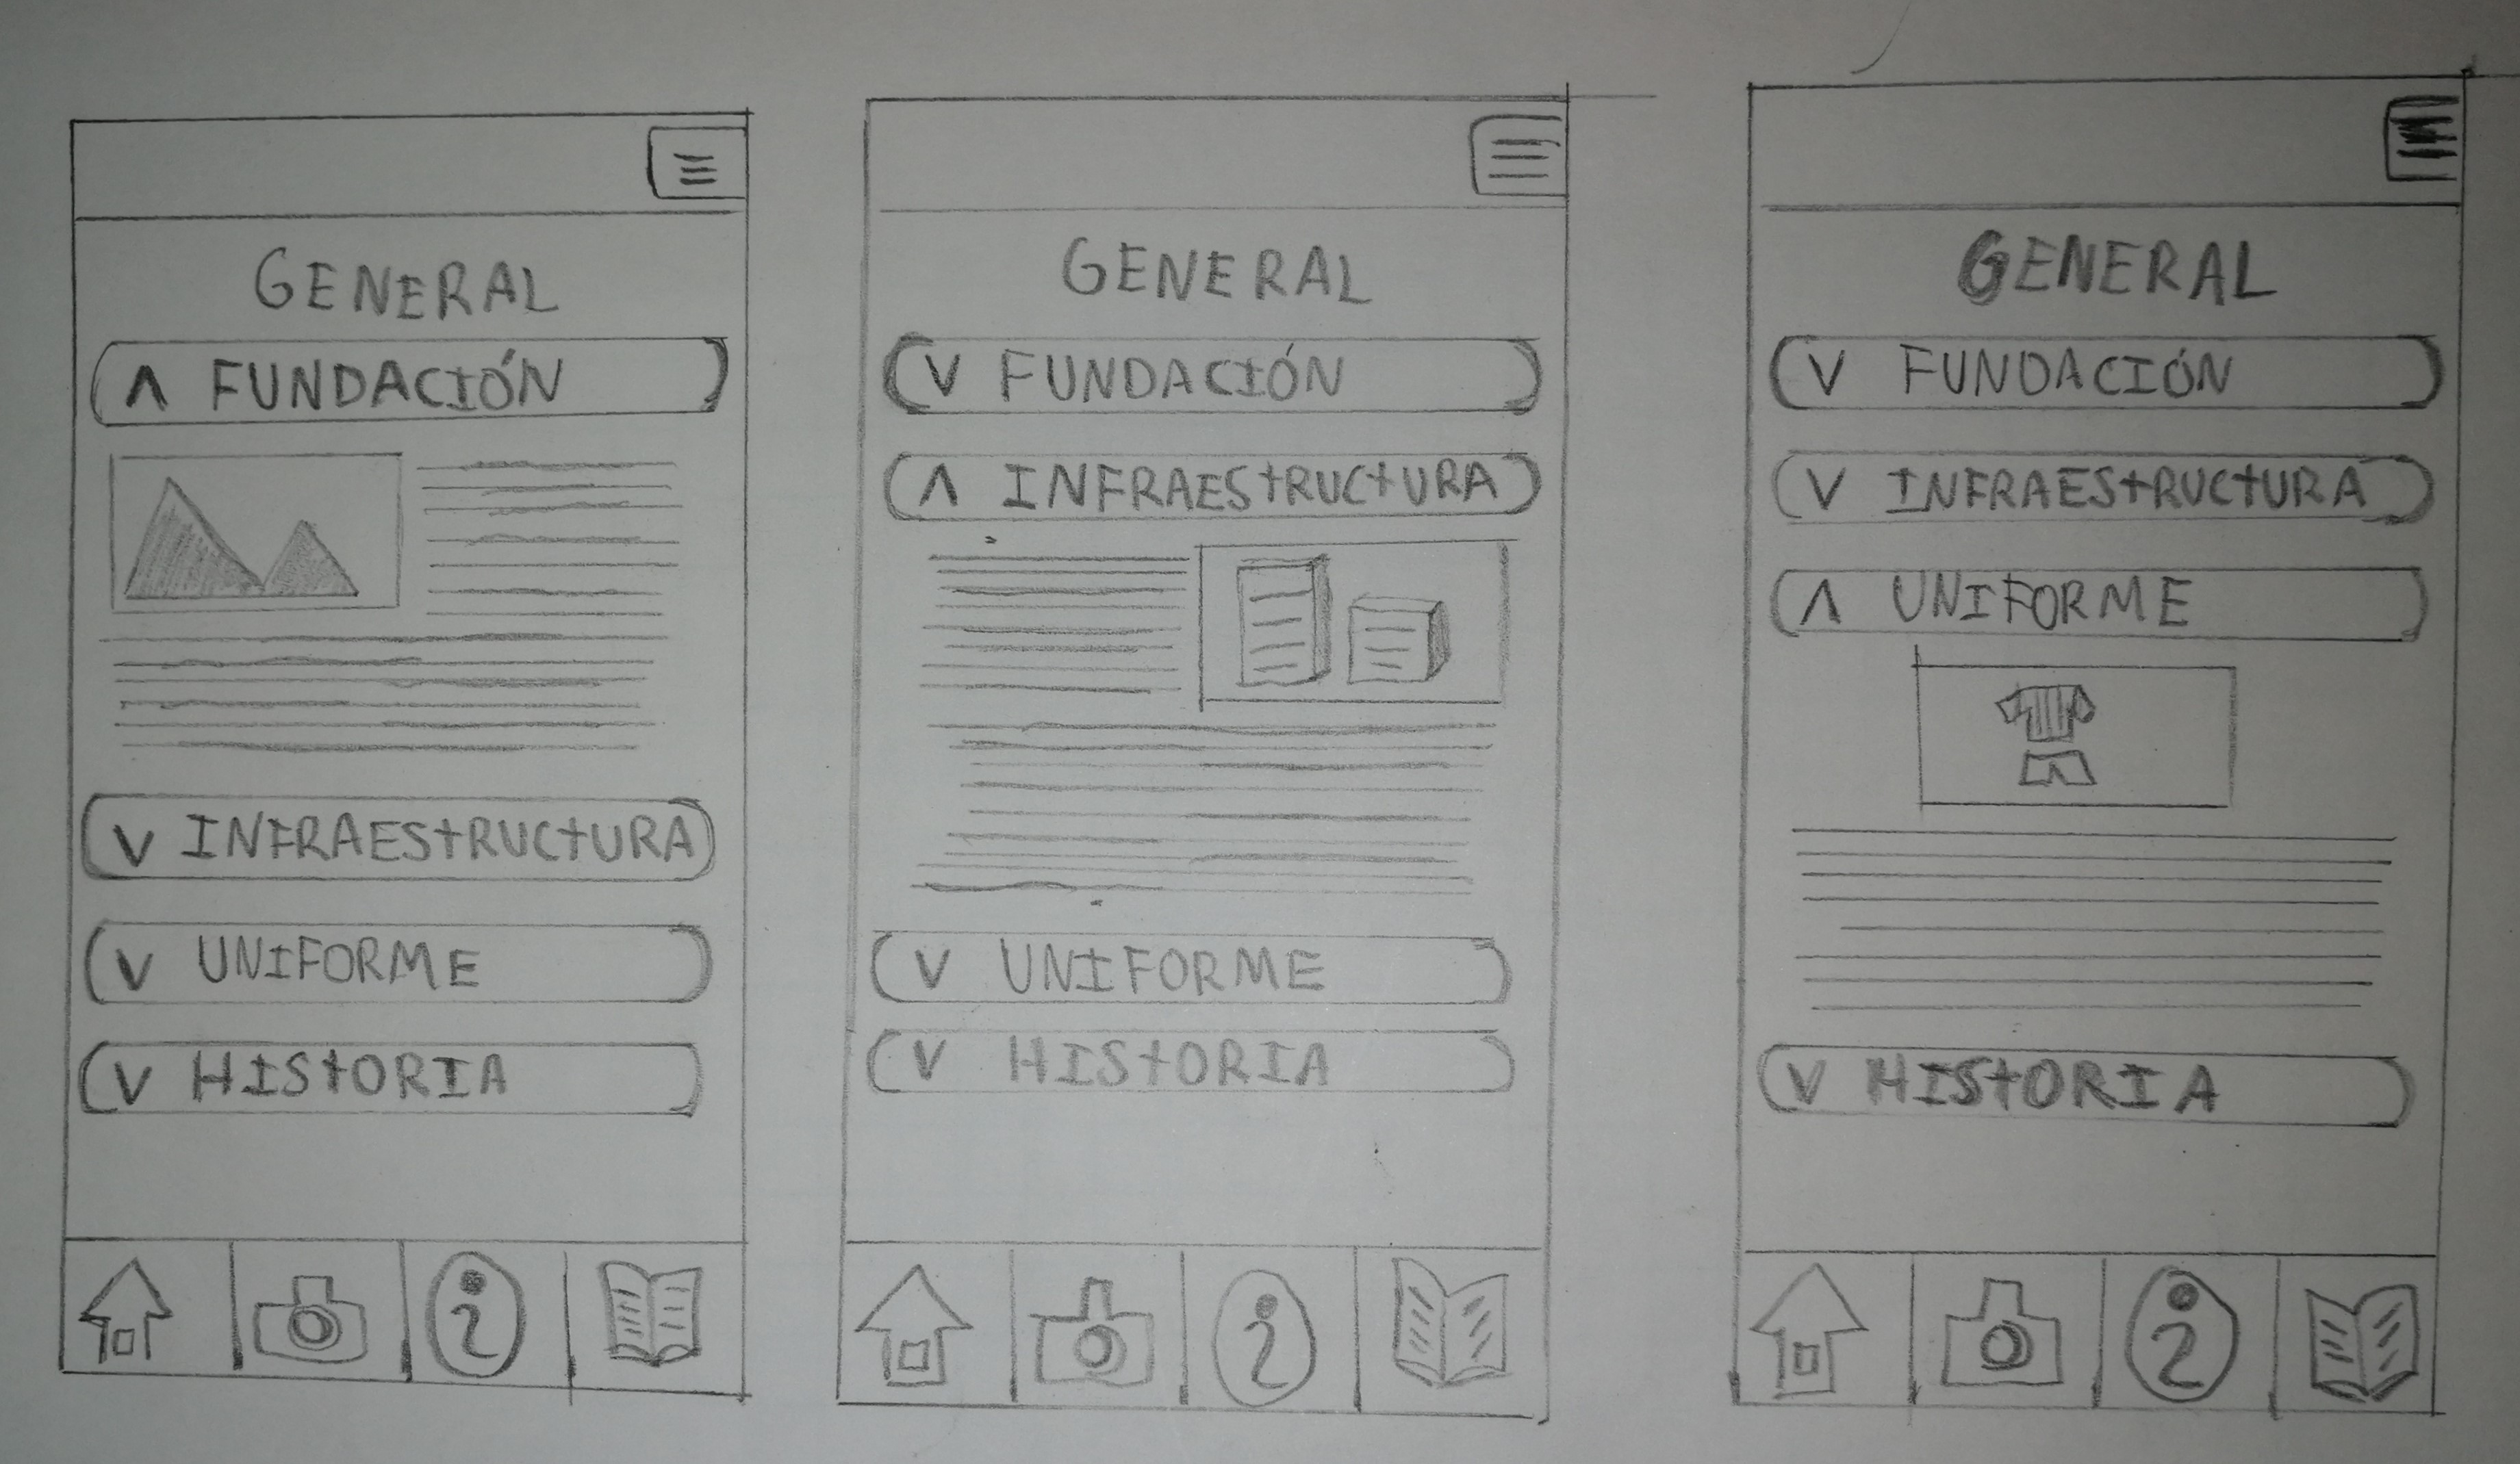
\includegraphics[width=\linewidth]{copia_all.jpg}
   \caption{Informacion General.}

    \caption{The same cup of coffee. Multiple times.}
   \end{figure}
\end{frame}
\section{Historias del Equipo}
\begin{frame}{Historias del Equipo}
%\textcolor{red}{Prototipo TradeOff:}\textbf{ (Información vs tiempo)}
\begin{figure}
\centering
   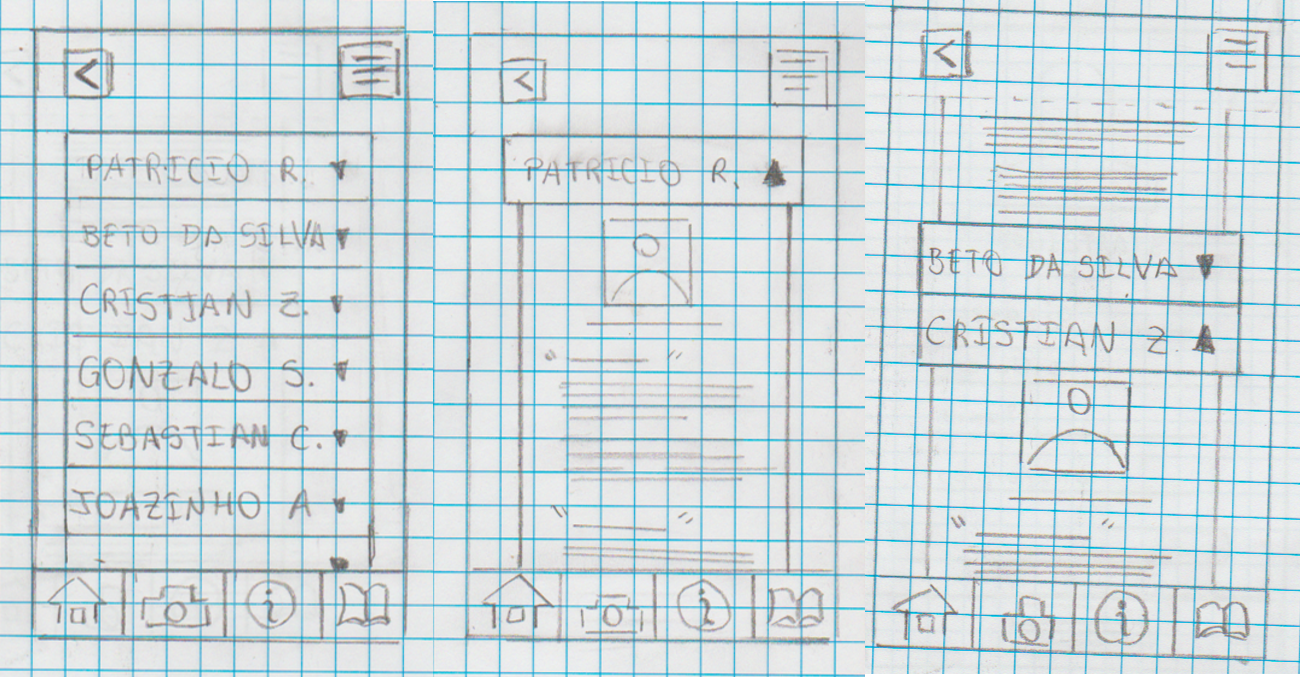
\includegraphics[width=\linewidth]{trabajo.png}
   \caption{Historias por jugadores}
\end{figure}
\end{frame}
\section{Inicio de sesión, registro y partidos del equipo}
\begin{frame}{Inicio de sesión, registro y partidos del equipo}
\begin{figure}
    \centering
    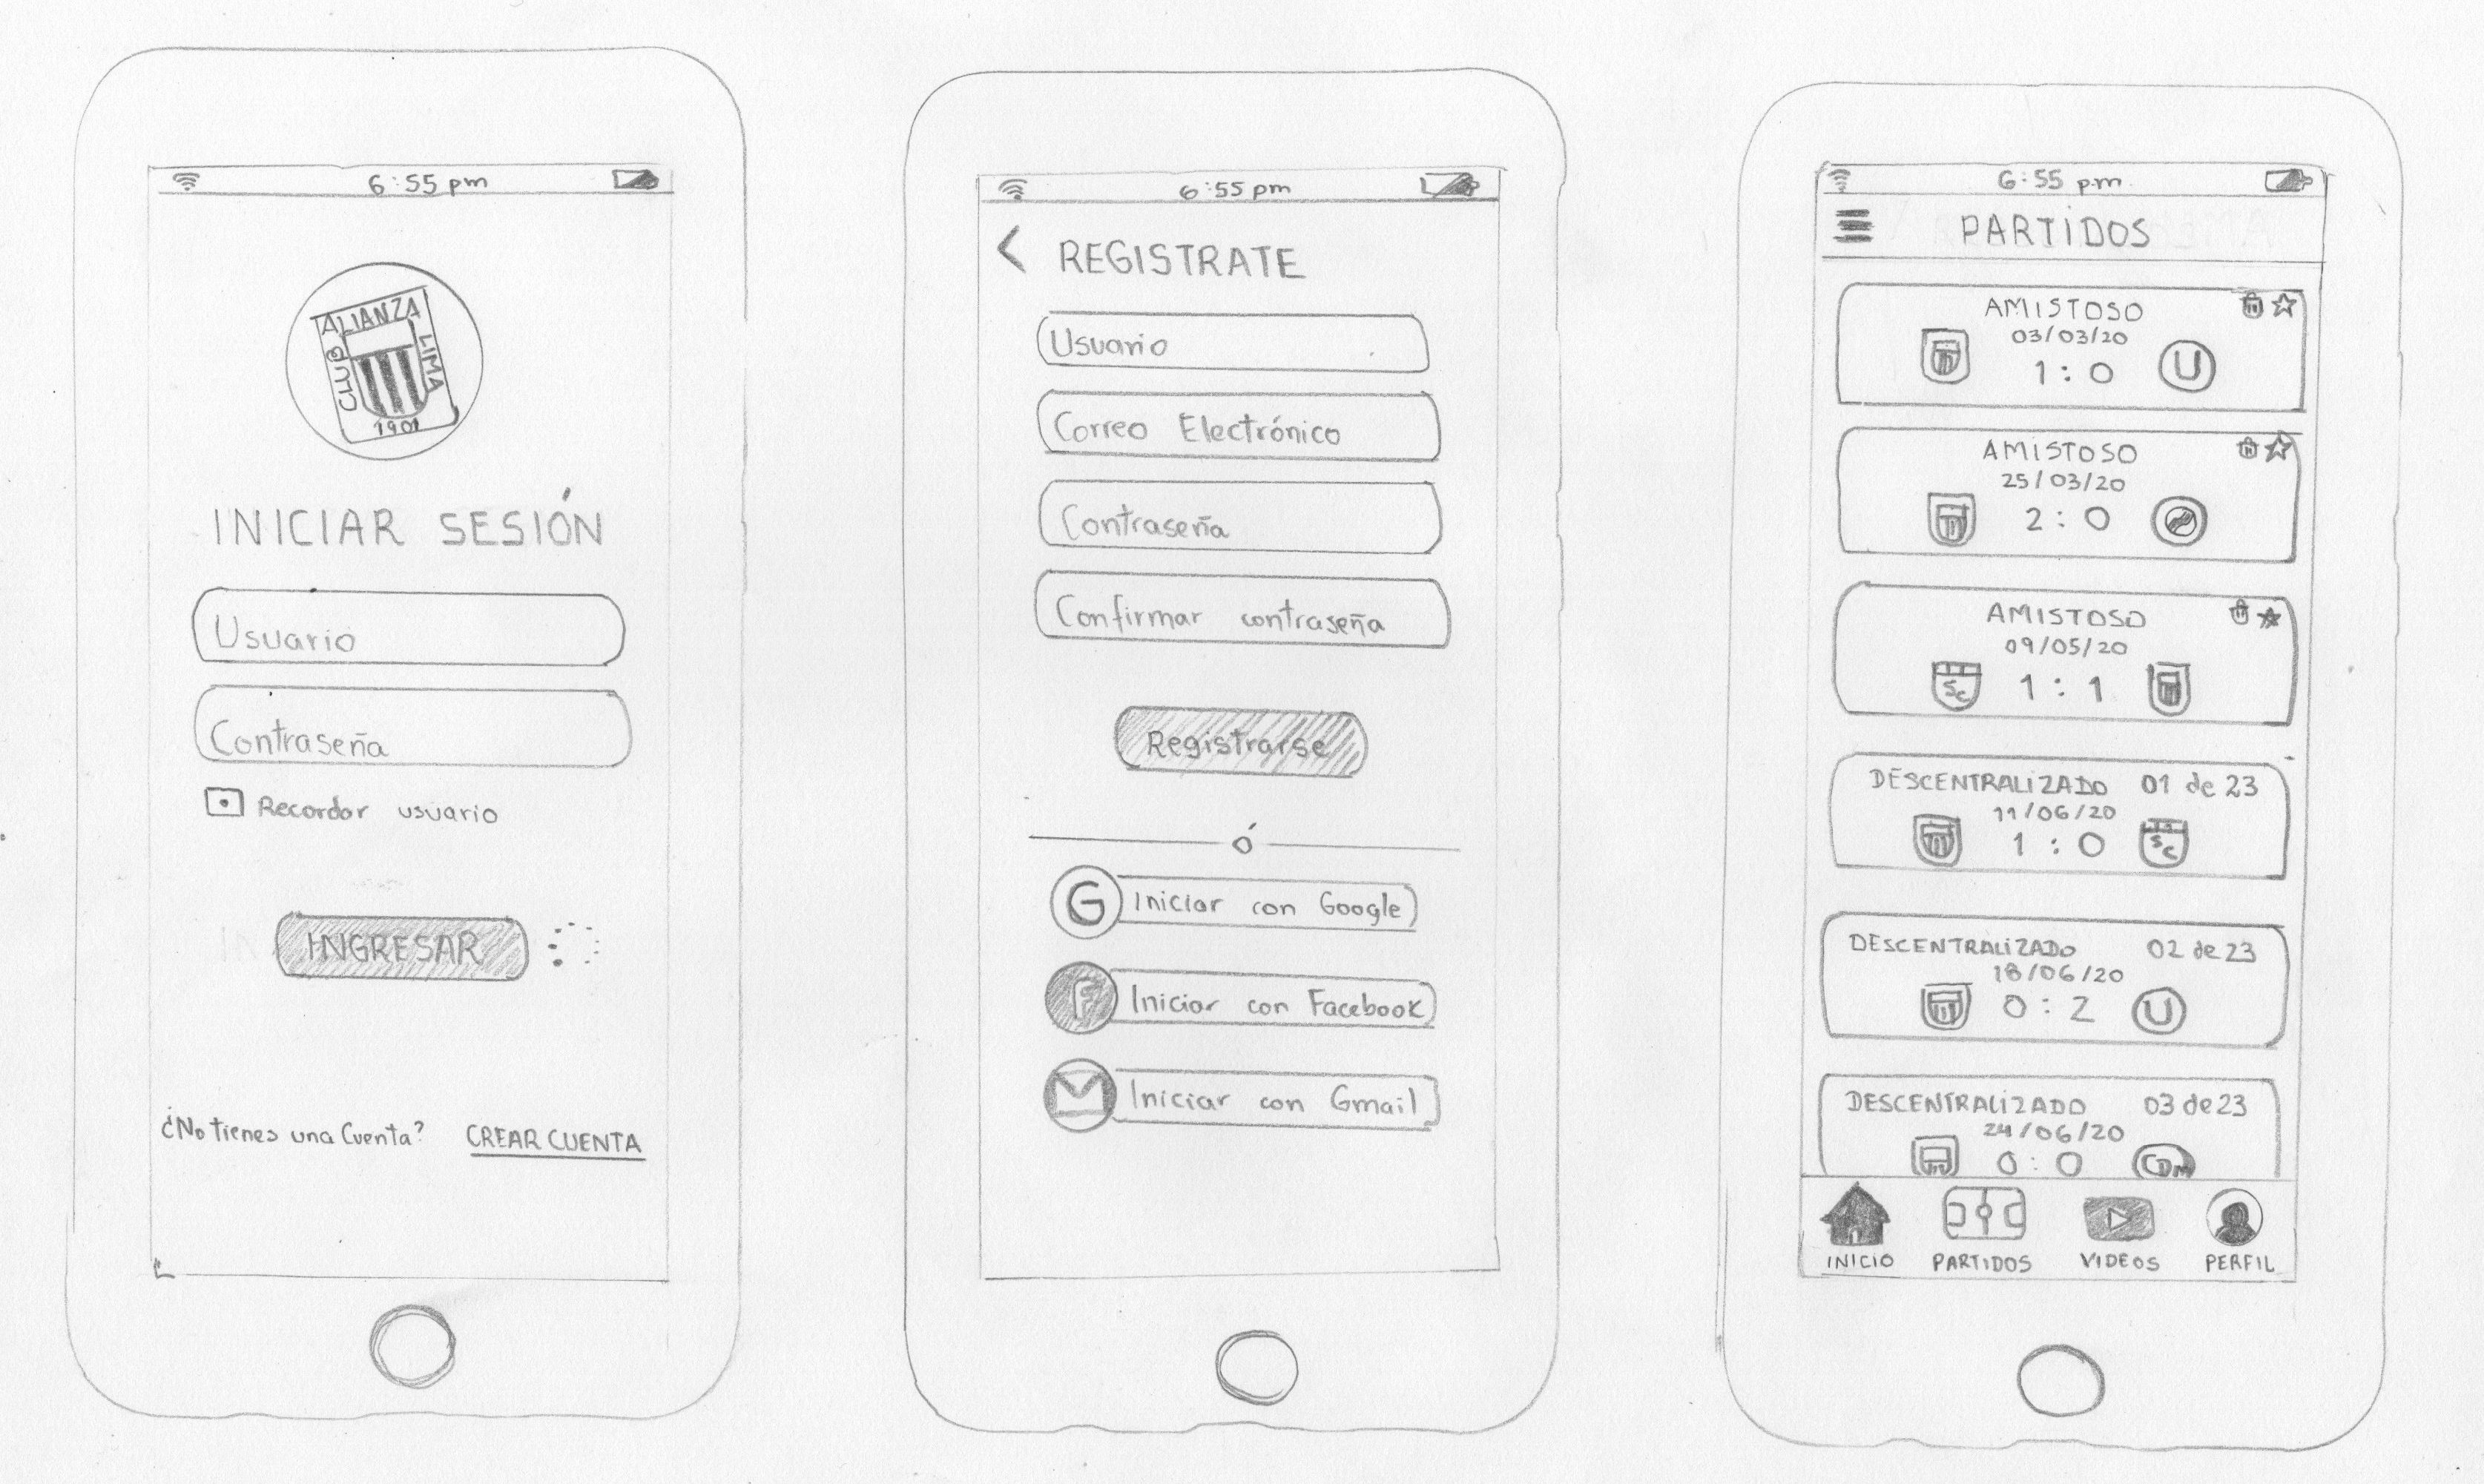
\includegraphics[width=\linewidth]{ihc002.jpg}
\end{figure}
\end{frame}
\section{Actualizaciones y partidos del equipo}
\begin{frame}{Actualizaciones y partidos del equipo}
\begin{figure}
  \centering
  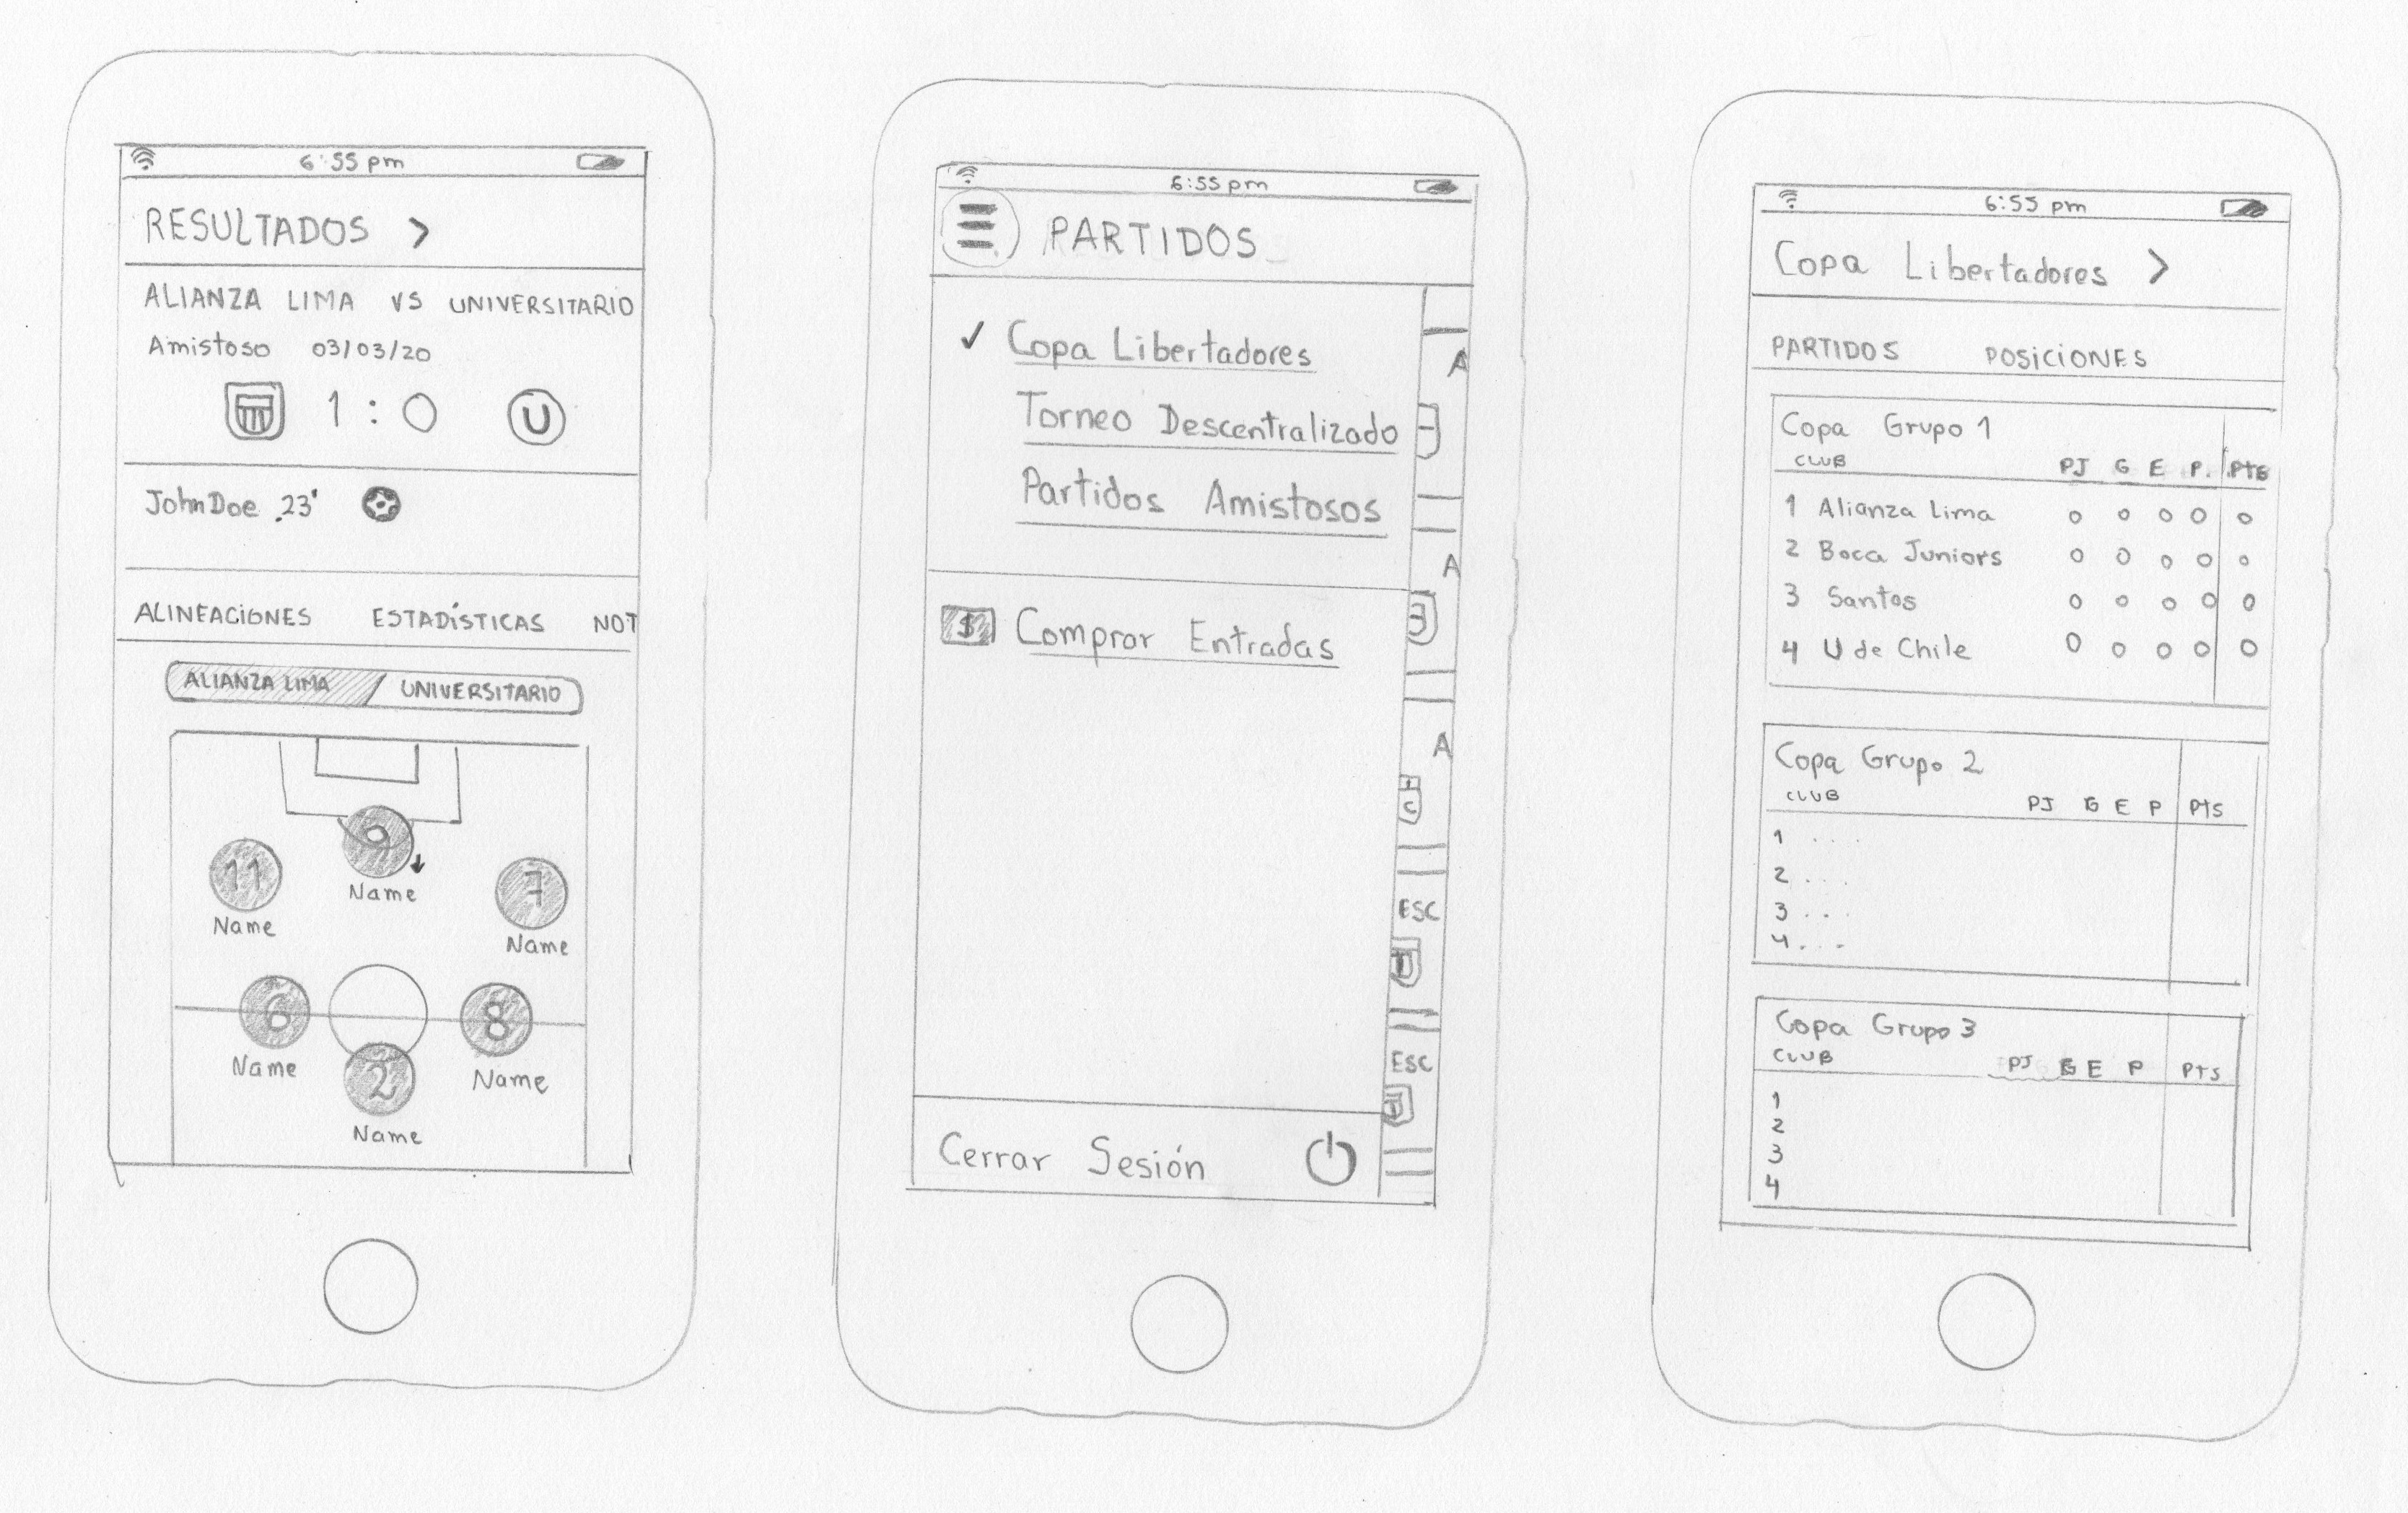
\includegraphics[width=\linewidth]{ihc003.jpg}
\end{figure}
\end{frame}

\section{References}
%References frame
\begin{frame}
\frametitle{References}
\begin{itemize}
%que titulo le pongo?
%prototipado en papel?que?? ahhh si ponle esook
\item Daves.M Paper Prototyping as a Core Tool in the Design of Cell Phone User Interfaces(http://www.id-book.com/casestudy-11-1-2.php).
\end{itemize}
\end{frame}

\end{document}